\documentclass[letterpaper,12pt]{article}

%math and margin packages
\usepackage{amsmath,amsfonts,amssymb,amsthm}
\DeclareMathOperator{\sech}{sech}
\usepackage{braket}
\usepackage[margin=1.0in]{geometry}
\usepackage{bbold}
\usepackage{braket}
\usepackage{ragged2e}
\usepackage{tikz}
\usetikzlibrary{angles,quotes}
\usepackage{tkz-euclide}
\usepackage{svg}
\usepackage{setspace}
\usepackage{physics}
\usepackage{hyperref}
\usepackage{float}
\allowdisplaybreaks
\doublespacing

\usepackage{titling}
\renewcommand\maketitlehooka{\null\mbox{}\vfill}
\renewcommand\maketitlehookd{\vfill\null}

\title{
\normalfont \normalsize 
\textsc{APPM 2360 - Intro Diff Eq W/Lin Alg \hfill Fall 2024} \\
[10pt] 
\rule{\linewidth}{0.5pt} \\[6pt] 
\huge Project 1 - Fish Population Modeling \\
\rule{\linewidth}{2pt}  \\[10pt]
}
\date{October 08, 2024}
\author{Daniel Alemayehu, Eli Grundberg}

\begin{document}
\begin{titlingpage}
\maketitle
\end{titlingpage}

\newpage

\section{Introduction}
We interested in stocking a local suburban neighborhood pond with a species of trout such that people can enjoy finishing in said pond. 
However, we want to prevent the pond from being overfished. 
More specifically, we want to make sure there is always fish in the pond such that anyone who goes fishing has a nonzero chance of catching a fish. 
To accomplish this, we'll analyze Rainbow, Brown, and Brook trouts to see which population allows for the most amount of trout to be harvested. 
In other words, we'll maximize the rate of harvesting of trout.
\section{Trout Population Model}
In order to determine the best species of trout to stock the lake with we analyzed the following modified logistic population model below:
\begin{equation} \label{eq:1}
    \dv{y}{t} = r\left(1 - \frac{y}{L}\right)y - h(y)
\end{equation}
This differential equation models the growth of the fish population in hundereds of fish per month. 
\begin{itemize}
    \item \(r\) is representative of our intrinsic growth rate of the fish population, as a unitless percent quantity representing how much the population grows by.
    \item \(L\) is representative of the carrying capacity, or the maximum fish population, in units of hundreds of fish.
    \item \(h(y)\) is the rate the people harvest trout from the pond as a function of hundreds of fish defined below as:
\end{itemize}
\begin{equation} \label{eq:2}
    h(y) = \frac{py^2}{q + y^2}
\end{equation}
Where \(p\) relates the number of people fishing and \(q\) relates the temperature of the water.
This also implies Equation \eqref{eq:1} is an autonomous differential equation denoting that our logistic curve of our fish population exists independently of when we stock the lake with trout. 
More specifically, our model does not account for any seasonal effects or orther temporal effects that may influence the trout population or the rate of harvest.
\section{Qualitative Analysis}
\subsection{Trout Population Growth}
To begin the qualitative anaylsis of the model we'll consider the logistic growth section of Equation \eqref{eq:1} defined as:
\begin{equation*}
    \dv{y}{t} = r\left(1 - \frac{y}{L}\right)y
\end{equation*}
Where the general solution can be analytically found as:
\begin{equation} \label{eq:3}
    y(t) = \frac{L}{1 + \left(\frac{L}{y_0} - 1\right)e^{-rt}}
\end{equation}
We'll consider a variety of trout species with varying carrying capacities but the same intrinsic growth rate by graphing the specific solution of Equation \eqref{eq:3} where the following is set:
\begin{itemize}
    \item \(r = 0.65\).
    \item \(t \in [0,15]\).
    \item \(y(0) = 1\).
    \item \(L = 5.4\) is the carrying capacity for Rainbow Trout.
    \item \(L = 8.1\) is the carrying capacity for Brown Trout.
    \item \(L = 16.3\) is the carrying capacity for Brook Trout.
\end{itemize}
Below is the graph of the specific solution:
\newline
\begin{figure}[H]
    \centering
    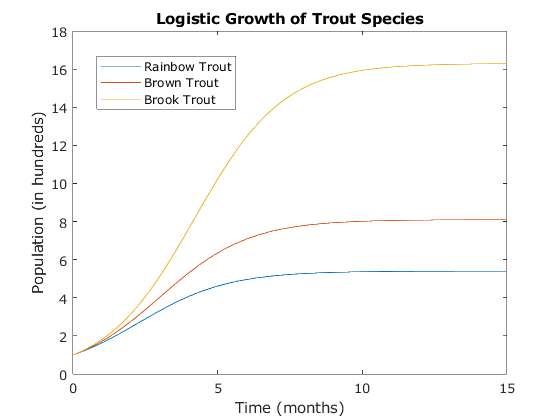
\includegraphics{./figures/fig.3.2.1.png}
    \caption{Trout Populations modelled by the Specific Solution, Code in Appendix}
    \label{fig:1}
\end{figure}
As expected on the graph the Trout species approch their respective carrying capacities as \(t \to \infty\) and when \(t \to 0\), \(y = y_0 = 1\).
A better point of comparison is \(t = 6\) for 6 months.
At \(t = 6\), the unharvested Rainbow species is expected to nearly reach it's carrying capacity where it's currently at 500 fish.
Meanwhile at \(t = 6\), the Brown Trout is expected to reach a population of around 700 Trout.
And for the Brook Trout, at \(t = 6\), it reaches a population of aroung 1250 fish.
This point of comparison shows how quickly the Rainbow and Brown Trouts are going to reach their carrying capacities, in comparison to the Brook Trout.
\subsection{Neighborhood Havesting}
The next part of qualitative analysis is observing how the harvesting function, Equation \eqref{eq:2} changes in relation to the trout population and different constants for \(p\) and \(q\).
To best visualize this we'll consider \(y \in [0,10]\) and varying values of \(p,q \in \{1, 1.5, 2\}\) as graphed below.
\newline
\begin{figure}[H]
    \centering
    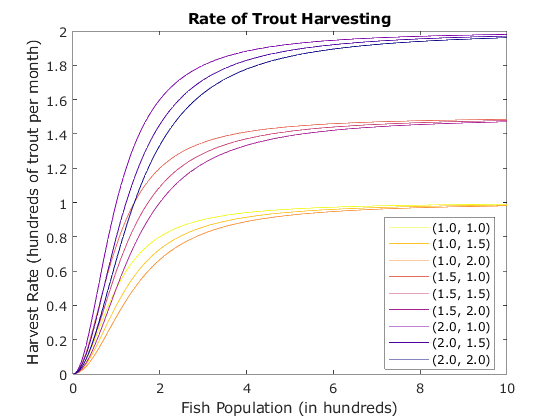
\includegraphics{./figures/fig.3.3.1.png}
    \caption{In our legend \(p\) and \(q\) are annoted as a tuple \((p,q)\), Code in Appendix}
    \label{fig:2}
\end{figure}
From Figure \eqref{fig:2} we can derive two important behaviors about the rate of trout harvest.
\begin{enumerate}
    \item As Trout populations approach 0 no havesting can occur.
    \item As Trout populations approach large numbers, the rate of harvesting is limited by the number of people.
\end{enumerate}
Analytically, if we observe the limit of the harvesting function as \(y\to 0\) and \(y\to \infty\) this confirms our two observations from our graph (See Appendix ? for specific calculations). 
Physically, this would also appear to make sense considering that if there were no fish left to harvest then the rate of harvest would be 0. 
If there was a very large population of fish, the amount of fish harvested would depend on how many people are harvesting since people can only harvest a finite amount of fish from a very large Trout population at a given time.
\subsection{Population Stability}
The final part to the qualitative analysis is to analyze the equilibrium solutions of Equation \eqref{eq:1}. The "equilibrium solutions" will help identify \(y\) values for which the population of trout tends towards or is tenously balanced at. We'll graph \(\d{y}{t} = f(y)\) for the following conditions:
\begin{itemize}
    \item \(y \in [0, 15]\)
    \item \(p = 1.2\)
    \item \(q = 1.0\)
    \item \(r = 0.65\)
    \item \(L = 5.4\) for Rainbow Trout
    \item \(L = 8.1\) for Brown Trout
    \item \(L = 16.3\) for Brook Trout
\end{itemize}
\begin{figure}[H]
    \centering
    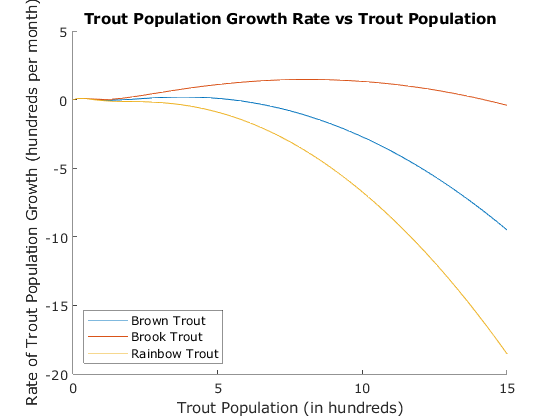
\includegraphics{./figures/fig.3.4.1.png}
    \caption{Code in Appendix}
    \label{fig:3}
\end{figure}
The roots are a little bit difficult to precisely identify at a first glance on the graph so we can also apply rootfinding algorithms (code in Appendix) to identify the roots of the above function more closely. 
The graphs are still helpful because the root finding algorithms can only find a single root so specifiying a range where the root occurs helps to identify the root we're interested in.
The roots for each curve are approximated below:
\begin{itemize}
    \item For Rainbow Trout: \(f(y) = 0\) for \(y \in \{0, 0.7050\}\).
    \item For Brown Trout: \(f(y) = 0\) for \(y \in \{0, 0.8018, 1.8564, 5.4418\}\).
    \item For Brook Trout: \(f(y) = 0\) for \(y \in \{0, 14.1898\}\).
\end{itemize}
The significance of the roots is that they denote equilibrium solutions, where the change in the Trout population is 0 since we're graphing the rate of change of the Trout population as a function of the Trout population.
Another tool we can use to identify equilibrium solutions is the direction field, which will help visualize the curve of the Trout Population function and the stability of the equilibrium solutions.
Below direction fields for each Trout species is modelled:
\begin{figure}[H]
    \centering
    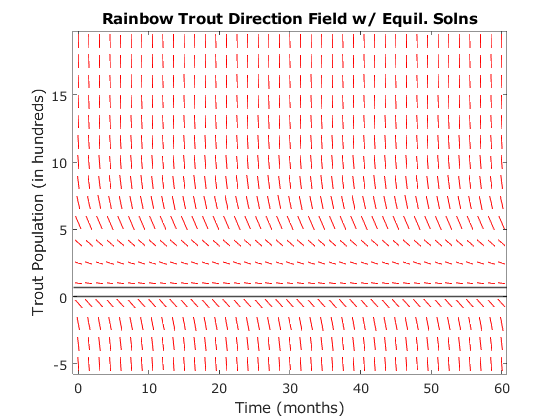
\includegraphics{./figures/fig.3.4.4.png}
    \caption{Code in Appendix}
    \label{fig:4}
\end{figure}
\begin{figure}[H]
    \centering
    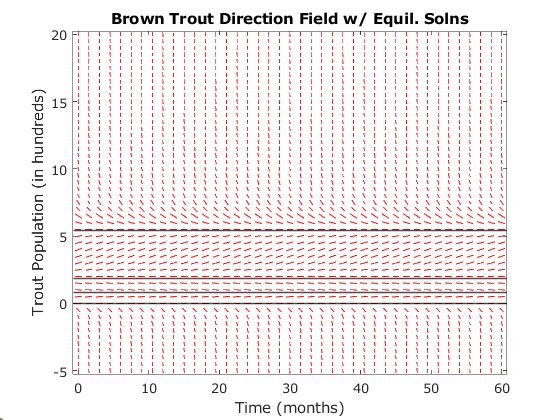
\includegraphics{./figures/fig.3.4.2.png}
    \caption{Code in Appendix}
    \label{fig:5}
\end{figure}
\begin{figure}[H]
    \centering
    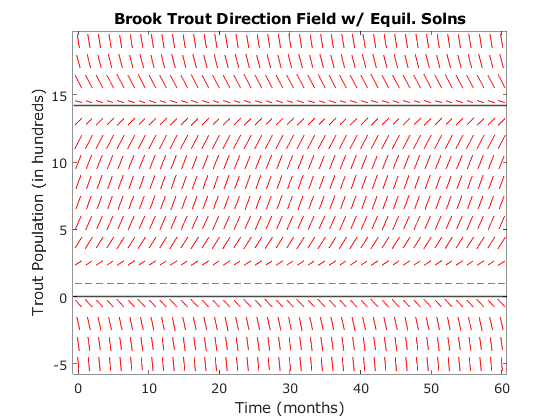
\includegraphics{./figures/fig.3.4.3.png}
    \caption{Code in Appendix}
    \label{fig:6}
\end{figure}
Some interesting things to note above:
\begin{itemize}
    \item For all graphs \(y = 0\) is an unstable solution, specifically, all solutions tend away from \(y = 0\).
    \item The Brown trout the only species with 4 equilibrium solutions, 2 stable, 2 unstable 
        \begin{itemize}
            \item \(y = 0\) is unstable as previously mentioned.
            \item \(y = 0.8018\) is stable for Brown Trouts.
            \item \(y = 1.8564\) is unstable for Brown Trouts.
            \item \(y = 5.4418\) is stable for Brown Trouts.
        \end{itemize}
    \item The Rainbow Trout has only one stable equilibrium and it's at a small value for the population.
    \item The Brook Trout may have a semi-stable solution at \(y = 1\)?
    \item No Trout Species can ever go extinct because for all \(y > 0\) the solution tends towards a positive equilibrium state.
    \item The Brook Trout population always approaches it's maximal stable equilibrium 
\end{itemize}
\section{Numerical Analysis} 
To get a better grasp of the Trout Population in relation to harvesting by the neighborhood, we can also apply Euler's method to approximate the fish population at a given time. 
We'll utilize Equation \eqref{eq:1} to identify our slope for Euler's Method with the following conditions as well:
\begin{itemize}
    \item \(p = 1.2\)
    \item \(q = 1.0\)
    \item \(r = 0.65\)
    \item Euler step size \(h = 0.01\)
    \item \(t \in [0,80]\)
    \item \(L = 5.4\) for Rainbow Trout
    \item \(L = 8.1\) for Brown Trout
    \item \(L = 16.3\) for Brook Trout
    \item We'll test \(y(0) \in \{0.5,1,2,20\}\) respectively on new plots for different inital conditions.
\end{itemize}
\begin{figure}[H]
    \centering
    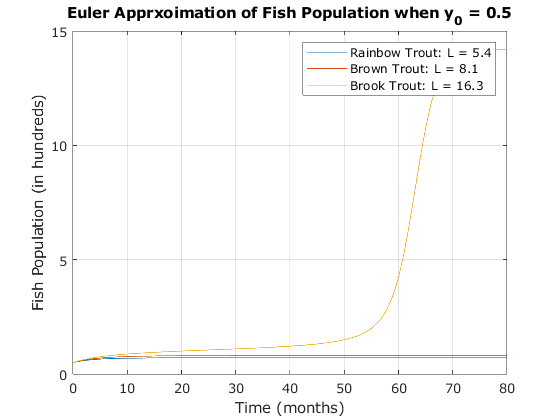
\includegraphics{./figures/fig.4.1.1.png}
    \caption{Code in Appendix}
    \label{fig:7}
\end{figure}
\begin{figure}[H]
    \centering
    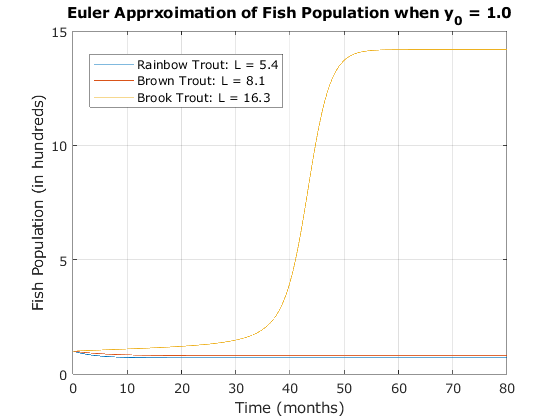
\includegraphics{./figures/fig.4.1.2.png}
    \caption{Code in Appendix}
    \label{fig:8}
\end{figure}
\begin{figure}[H]
    \centering
    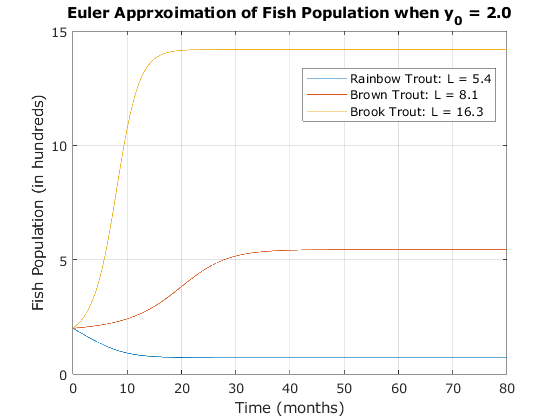
\includegraphics{./figures/fig.4.1.3.png}
    \caption{Code in Appendix}
    \label{fig:9}
\end{figure}
\begin{figure}[H]
    \centering
    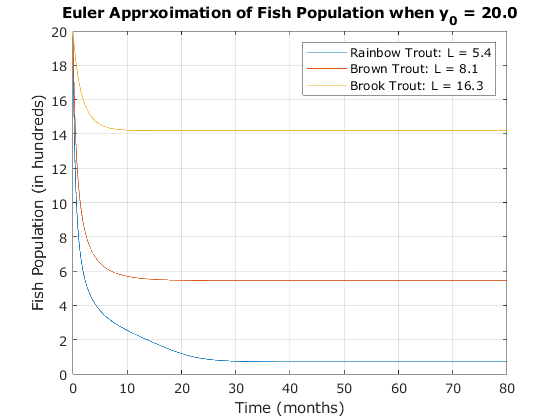
\includegraphics{./figures/fig.4.1.4.png}
    \caption{Code in Appendix}
    \label{fig:10}
\end{figure}
\begin{itemize}
    \item For the Rainbow Trout, all tested inital conditions result in the Trout species nearly dying out.
    \item For the Brown Trout, inital condtions \(y(0) \in \{2, 20\}\) resulted in the species reaching it's population capacity given the harvest rate
    \item For the Brook Trout, all test inital conditions proved irrelevant to the trout species eventually reaching it's population capacity given the harvest rate
\end{itemize}
\section{Conclusion}
In conclusion, we can choose a species to stock the lake given a variety of conditions.
\begin{itemize}
    \item If we want to stock the lake while staring with the fewest fish possible we should choose the Brook Trout since their species can accomidate the most harvesting because their species usually reaches near their carrying capacity.
    \item If we want to stock the lake....
    \item Either way for any species we won't overfish the lake so choosing based on that criterion is largely irrelevant.
\end{itemize}
But our model doesn't account for a critical array of information. 
For starters, we'll likely need to stock the lake with prey for the fish as well so they don't die out whiel being fished and that may effect how much of the Trout can reside in the lake.
We also don't take into account any season or other temportal related effects into our model when stocking the lake.
Stocking the lake in winter may prove detrimental to the fish population while stocking during spring mating season will allow for the fish population to grow much faster.
Finally, it would also be worthwhile to consider stocking the lake with a mixture of Trout species if they are not predators of each other.
Having variety in the lake will make fishing a lot more fun, especially with smaller populations like the Rainbow Trout fitting well into a fabled catch archetype for the neighborhood.
\section{Appendix}
MFW filling appendix :(
\end{document}
